\documentclass[12pt]{article}
\usepackage[a4paper, total={7.5in, 10in}]{geometry}
%\usepackage{array}
\usepackage{graphicx, subfig, wrapfig, fancyhdr, lastpage, multicol ,color}
\newcommand\headerMe[2]{\noindent{}#1\hfill#2}
\usepackage[mathscr]{euscript}

\setlength{\columnseprule}{1pt}
\def\columnseprulecolor{\color{blue}}


\pagestyle{fancy}
\fancyhf{}

\cfoot{\em{Page \thepage \hspace{1pt} / \pageref{LastPage}}}
\begin{document}

\headerMe{Royaume du Maroc}{année scolaire \emph{2021-2022}}\\
\headerMe{Ministère de l'Éducation nationale, }{  Professeur :\emph{Zakaria Haouzan}}\\
\headerMe{du Préscolaire et des Sports}{Établissement : \emph{Lycée SKHOR qualifiant}}\\

\begin{center}
Devoir Surveillé  N°1 \\
    Filière 1Bac Sciences Mathématiques\\
Durée 2h00
\\
    \vspace{.2cm}
\hrulefill
\Large{Chimie 7pts/42min}
\hrulefill\\

    %\emph{Les questions parties sont indépendantes}
\end{center}
%end Headerss------------------------
%__________________Chimie ______________________-
%%%%%%%+_+_+_+_+_+_+_+_+_Partie1

 \section*{Partie 1 :Les comprimés effervescents de Vitamine B5 \dotfill(3.5pts) }
 
 Les comprimés effervescents de Vitamine B5, contiennent acide pantothénique $C_9H_{17}NO_5$ et le
   pantothénate de sodium $NaC_9H_{16}NO_5$ est le sel de sodium de la vitamine B5 , ce dernier est
employé comme additif alimentaire.

\begin{enumerate}

  \item Écrire l’équation de dissolution de pantothénate de sodium dans l’eau. \dotfill(0.5pt)

  \item Identifier le couple acide / base mettant en jeu l’acide pantothénique et écrire la demi-équation acido-basique correspondante.\dotfill(1pt)

\item  On fait réagir une masse m = 3,00 g d’acide pantothénique avec 150 mL d’une solution
d’hydroxyde de sodium $(Na^+, HO^-)$de concentration $C=2,50.10^{-1} mol.L^{-1}$.
    \begin{enumerate}
      \item Identifier les couples acide / base mis en jeu, puis écrire l’équation de la réaction envisagée.\dotfill(1pt)

      \itemÉtablir un tableau d’avancement et déterminer l’avancement maximal de la réaction. Quel est
        le réactif limitant ?\dotfill(1pt)
    \end{enumerate}
\end{enumerate}
\section*{Partie 2 : L’eau de javel \dotfill(3.5pts) }

L’eau de javel est une solution aqueuse d’hypochlorite de sodium de formule $(Na^+_{(aq)} + ClO^-_{(aq)} )$.
La formule chimique d’une solution aqueuse d’acide chlorhydrique $(H_3O^+,Cl^-)$
\begin{enumerate}
  \item Écrire les demi-équations électroniques des deux couples suivants : $ClO^-/Cl_2$ et $Cl_2 /Cl^-$. \dotfill(0.5pt)
    
  \item  Écrire l’équation de la réaction entre les ions chlorure et hypochlorite. \dotfill(1pt)
  
  \item Soit $250mL$ d’eau de Javel contenant une quantité de matière d’ions hypochlorite $n(ClO^-)=0,41mol$ a été mélangée avec un détartrant à base d’acide chlorhydrique dans une pièce de volume $V=3,5 m^3$ .
    \begin{enumerate}
 \item Établir le tableau d’avancement relatif à la transformation chimique précédente. On considèrera que les ions $H^+_{(aq)}$ et $Cl^-_{(aq)}$ ont été introduits en excès. \dotfill(0.75pt)

 \item Calculer la quantité de matière $n$ du gaz toxique produite. \dotfill(0.75pt)
 \item En déduire le volume V de gaz toxique dégagé à 20°C et à pression atmosphérique normale. \dotfill(0.5pt)
   \end{enumerate}
\end{enumerate}

 %_____________________________________PHYSIque Partie 22222____________________________________________________________________________
\begin{center}
    \vspace{2cm}
\hrulefill
\Large{Physique 13pts - 78min}
\hrulefill\\
    \emph{Les parties sont indépendantes}
\end{center}
%end Headerss------------------------
 \section*{Partie 1 : Champ électrique créé par une charge ponctuelle \dotfill(7pts)}

Sur un axe $(Ox)$, se trouve deux charges de valeurs $q_B = 2q_A = 2\mu C$ , On place $q_A$ dans l'origine O (A=O) ,les points A et B
distants d’une distance $AB=a=8 cm$, on donne $k = 9.10^9SI$

\begin{enumerate}
    \item  Soit un point $M \in AB$ d’abscisse $x$.
      \begin{enumerate}
        \item Montrer que l’expression du vecteur champ électrostatique en M est :\dotfill(2pt) $$\vec{E}(M) = kq_A.(\frac{1}{x^2} - \frac{2}{(a-x)^2})\vec{u}$$
        \item Déduire ses caractéristiques au point d’abscisse $x=2 cm$. \dotfill(1pt)
        \item Déterminer l’abscisse d’un point C où $E(C)=0$ .\dotfill(1pt)
      \end{enumerate}
    \item Donner les caractéristiques de $E(N)$ en un point $N$ d’abscisse $x_N =10 cm$. \dotfill(1pt)
    \item On remplace la charge $q_A$ par une charge $q’<0$ , déterminer la valeur de q’ pour que le champ électrostatique global s’annule en N. \dotfill(2pt)
\end{enumerate}

 \section*{Partie 2 : Principe de fonctionnement d'un oscilloscope \dotfill(6pts)}
Dans le canon à électrons d’un oscillographe (voir fig.), les électrons sortant de la cathode avec une vitesse
supposée nulle, sont accélérés par une tension U=1600V appliquée entre la cathode C et l’anode A.

1. Calculer en mètres par seconde la vitesse $v_A$ des électrons à la sortie du canon.\dotfill(1pt)
   
2. Calculer en joule et en kilo électronvolts, leur énergie cinétique $E_{CA}$\dotfill(1pt)
   \begin{center}
    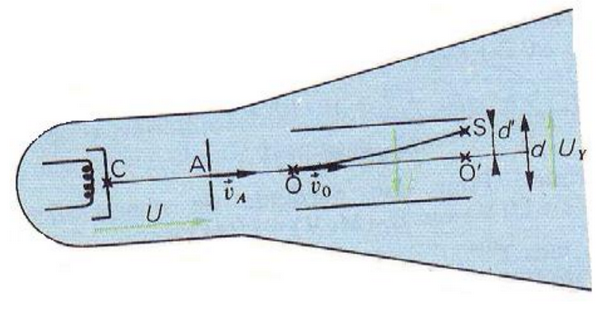
\includegraphics[width=0.5\textwidth]{./img/img_02.png}
      \end{center}
   3. Les électrons pénètrent avec une vitesse $V_O = V_A$, entre les plaques de déviation verticale, en un point O
situé à égale distance de chacune d’elles. Lorsque la tension $U_1 = 500V$ est appliquée à ces plaques
distantes de d = 2cm, les électrons sortent de l’espace champ en un point S tel que O’S=d’=0,6cm.
   \begin{enumerate}
     \item[a.] On prend l’origine des potentiels $V_0$ = 0 au point O. Calculer Vs potentiel électrostatique du point S del’espace champ.\dotfill(1pt)

     \item[b.] Déterminer Epo et Eps, énergies potentielles électrostatique d’un électron en O et en S dans l’espace champ, en joules et en kilo électronvolts.\dotfill(2pt)

     \item[c.] En déduire $Ec_s$ énergie cinétique de sortie des électrons, en kilo électronvolts.\dotfill(1pt)
   \end{enumerate}


\end{document}
